\section{Software}

EL Google Chromecast no es más que un dispositivo compatible con el protocolo propietario de Google Cast que actúa como receptor. Este protocolo fue lanzado en exclusividad para el Chromecast de primera generación en julio de 2013, pero en febrero de 2014 pusieron el SDK a disposición de los desarrolladores para usarlo en sus propias aplicaciones. En mayo de 2015 había más de 20.000 aplicaciones de terceros compatibles con esta tecnología según reconoce Google.

\

Para iniciar la reproducción de un contenido pulsamos el botón de \textit{cast}, que aparecerá automáticamente si Google Cast está integrado con la aplicación. En ese momento aparecen los dispositivos Chromecast conectados a la red local y se elige aquel donde se quiere emitir el contenido. Si el puerto HDMI dispone de Consumer Electronics Control (CEC) la televisión se encenderá inmediatamente.

\

Google Cast tiene dos modos de funcionamiento:

\begin{itemize}
	\item Uno es usar dispositivo desde el que solicitamos el streaming para controlar la reproducción (en adelante dispositivo emisor): pausar un vídeo, subir el volumen del audio, crear o modificar una cola de reproducción, etc.
	El dispositivo receptor (por ejemplo un Chromecast) es quien se encarga de descargarlo y comunicarse con el servidor de contenido, liberando al dispositivo emisor de esta tarea.
	Esto garantiza una carga de trabajo muy baja para el emisor y le permite estar bloqueado mientras la reproducción está teniendo lugar.
	El receptor ejecuta una versión adaptada del navegador Chrome para realizar el streaming.
	El contenido puede estar almacenado localmente en el dispositivo emisor o en un servidor externo.
	El primer caso ocurre en aplicaciones como Google Photos, mientras que un ejemplo del segundo serían Netflix o Youtube.
	Las aplicaciones emisoras que usen este modo de funcionamiento deben ser compatible con Android 4.1, iOS 7.0 o versiones superiores si son aplicaciones móviles y con Windows 7, macOS 10.7, Chrome OS 28 o versiones superiores si son aplicaciones Chrome.
	En este último caso, se debe tener instalada la extensión Cast.

	\item El otro modo es hacer mirroring de una pestaña de Chrome o del escritorio de un ordenador con Chrome o del de un dispositivo con Android 4.4 o superior.
	La calidad del streaming en este caso varía ampliamente según la potencia de procesamiento del emisor.
	En el caso de hacerse desde un smartphone, la calidad de las imágenes normalmente se deteriora debido al escalado.
\end{itemize}

Hasta diciembre de 2014, el dispositivo emisor y receptor debían estar conectados a la misma red Wi-Fi para reproducir contenido, pero en las versiones posteriores a esa fecha ya no es necesario.
Esto se debe a que se ha añadido un modo invitado.
En este modo, el receptor emite ultrasonidos a través de los altavoces y el emisor es capaz de localizarlo usando el micrófono.
Se usa un PIN de cuatro dígitos que aparece en pantalla para la verificación.
El modo invitado está disponible para todos los Chromecast con un dispositivo Android como emisor y para los Chromecast a partir de la segunda generación para aquellos con dispositivos iOS como emisor.

Según su propia documentacón, Google Cast implementa el paradigma del productor consumidor, tiene una aplicación que envía y otra que recibe.
\begin{itemize}
	\item La aplicación de envío ofrece controles para elegir el dispositivo de llegada.
	\item La aplicación receptora utiliza una aplicación web ejecutada en un entorno de Chrome del dispositivo. Se pueden hacer aplicaciones receptoras que aparte de soportar HTML5 tengan más variedad de protocolos de streaming: MPEG-DASH, HTTP Live Streaming, y Microsoft Smooth Streaming Protocol.
\end{itemize}

Chromecast para buscar dispositivos disponibles en una red Wi-Fi usa el protocolo mDNS (multicast Domain Name System), anteriormente usaba el protocolo DIAL (DIscovery And Launch).

Para la visualización de contenidos en la TV se mezclan conceptos DLNA (Digital Living Network Alliance) y Miracast\cite{DLNA-Miracast}.
A la hora de enviar contenido realmente se manda la orden a Chromecast de que reproduzca el contenido elegido directamente desde la nube.
Es la principal diferencia con DLNA, ya que no se reproduce contenido desde un servidor DLNA sino desde Internet.
Para usar solamente DLNA para streaming necesitaríamos aplicaciones de terceros, por ejemplo iMediaShare.
Otra funcionalidad es poder enviar los contenidos de una pestaña del navegador Chrome a la TV en lo que podríamos denominar una conexión Miracast pura y dura, punto a punto.




\begin{figure}[ht]
	\begin{minipage}[b]{0.55\linewidth}
	Utiliza un sistema operativo de escritorio llamado Chrome OS, siendo el navegador Google Chrome su principal herramienta de uso.
	Chrome OS se basa en el proyecto de código abierto Chromium OS,5 que, a diferencia de Chrome OS, se puede compilar a partir del código fuente descargado.
	\end{minipage}%%
	\begin{minipage}[b]{0.45\linewidth}
		\centering
		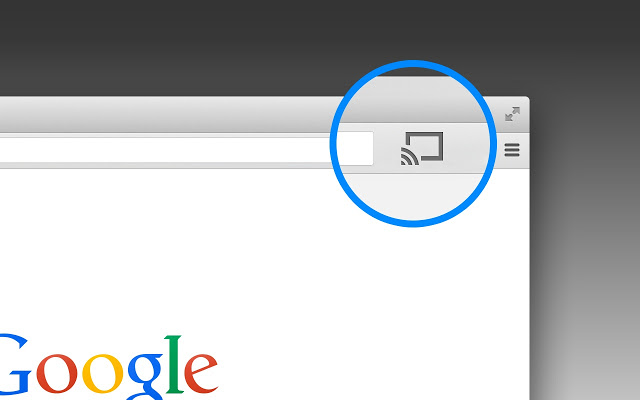
\includegraphics[width=.65\linewidth]{./Imagenes/googlecastbrowser.jpg}
	\end{minipage}
\end{figure}







\subsection{Google Cast}
\subsubsection{Google Home}

\subsection{mDNS (multicast Domain Name System)}


\subsection{Miracast}
Miracast es un protocolo multimedia para hacer streaming a un monitor desde un dispositivo local. Para que nuestra smartTV sea capaz de usarlo, necesita soportar Wi-Fi Direct. Wi-Fi Direct es una norma que permite la conexión entre dos dispositivos Wi-Fi sin necesidad de un intermediario.
Los dispositivos que envían y reciben información tienen que estar certificados para Miracast, pero existe un plug para dispositivos no certificados.
Miracast está disponible de manera nativa para dispositivos con versiones de Android 4.2 y Android 6.0.

\vspace{0.1cm}
\begin{figure}[ht]
	\begin{minipage}[b]{0.55\linewidth}
		La conexión está creada vía Wi-Fi Protected Setup (WPS), mecanismos para facilitar la configuración de una red WLAN con seguridad WPA2.
		WPS contempla cuatro configuraciones para el intercambio de credenciales: PIN (Personal Identification Number), PBC (Push Button Configuration), NFC (Near Field Communications) y USB (Universal Serial Bus). La configuración PIN no es recomendable por su debilidad ante ataques de fuerza bruta.
	\end{minipage}%%
	\begin{minipage}[b]{0.45\linewidth}
		\centering
		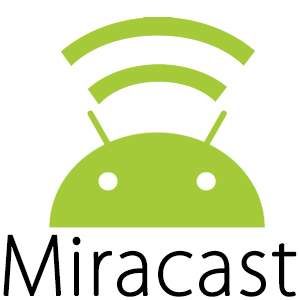
\includegraphics[width=.55\linewidth]{./Imagenes/miracast.jpg}
	\end{minipage}
\end{figure}

\

Para la capa de internet usa IPv4; para la de transporte, TCP/UDP, y para la de aplicación, RTSP y RTP, que se encargan de controlar el streaming.

\

A partir de Android 6.0, Google ha dejado de dar soporte nativo a Miracast en favor de su propio Google Cast.
Con Miracast el dispositivo receptor es dependiente de que el dispositivo Android emisor se mantenga activo \cite{Miracast}: si se bloquea también bloqueará la reproducción en el receptor.
Esto implica una mayor carga de trabajo y consumo de batería respecto a Google Cast, que solo se encarga de enviar señales para el control de la reproducción.

\

Existe una alternativa de código abierto a Miracast llamada MiracleCast. El nombre viene por la dificultad de crear una red Wifi-P2P estable (basado en wpa_supplicant).

\

El núcleo de MiracleCast es un demonio llamado miracled \cite{MiracleCast}, que controla links locales, las peticiones de conexión, se encarga de la codificación del protocolo y el parsing.
Su línea de comandos puede ser usada para controlar el demonio, crear nuevas conexiones, modificar parámetros, etc.
Soporta un modo interactivo que muestra las peticiones de conexión y permite al usuario aceptarlas o no.

\

El código fuente se puede encontrar en \href{https://github.com/albfan/miraclecast}{github}.



\subsection{Chrome OS?}
